\documentclass[dvipdfmx,11pt]{beamer}
\usepackage{pxjahyper}
\usepackage{minijs}
\usepackage{otf}
\usefonttheme{professionalfonts}
\setbeamertemplate{navigation symbols}{}
\renewcommand{\kanjifamilydefault}{\gtdefault}
\usetheme{Hannover}

\title{Python Program for Fictitious Play}
\subtitle{Matching Pennies Game}
\author{Tanaka Masaki}
\institute{The University of Tokyo}
\date{}

\begin{document}
\begin{frame}\frametitle{}
 \maketitle
\end{frame}

\section{Introduction}
\begin{frame}\frametitle{Introduction}
 \begin{itemize}
  \item Fictitious Playのシミュレーションプログラム
  \item 使用言語はPython
  \item プレイするゲームは``Matching Pennis Game''
 \end{itemize}
\end{frame}

\section{Fictitious Play}
\subsection{What's Fictitious Play?}
\begin{frame}\frametitle{What's Fictitious Play?}
 \begin{itemize}
  \item 戦略形ゲームが、$t= 1, 2, \ldots$の各期にプレイされる
  \item 他のプレーヤーの戦略に対する予測
  \begin{itemize}
   \item[→] $t$期の他のプレーヤーは、$1$期から$t-1$期に選択した分布に等しい確率で各純粋戦略を選択する
  \end{itemize}
  \item この予測の下で、各プレイヤーがそれに対する最適反応戦略を選択
  \item このような動学モデルを``Fictitious Play''と呼ぶ。
 \end{itemize}
\end{frame}

\begin{frame}\frametitle{What's Fictitious Play?}
 \begin{itemize}
  \item $t$期において、プレーヤー0は…
  \begin{itemize}
   \item[・] プレーヤー1が確率$1-x_{0}(t)$で行動0をとる
   \item[・] プレーヤー1が確率$x_{0}(t)$で行動1をとる
  \end{itemize}
  \item[] と予測しているものとする
  \item プレーヤー1に対しても同様
  \item この下で、期待利得が最大になるように行動を決定する(期待利得が等しい場合は等確率で選ぶ)
  \item なお、この$x_{0}(t)$を「プレーヤー0の、$t$時点におけるプレイヤー1の行動に関する信念(belief)」と呼ぶこととする
 \end{itemize}
\end{frame}

\begin{frame}\frametitle{What's Fictitious Play?}
 \begin{itemize}
  \item 初期信念$x_{0}(0)$は [0,1] 上の一様分布に従ってランダムに与えられる。
  \item 各$t \geq 1$時点において、プレーヤー1が過去とった行動を$a_{1}(0), \ldots ,a_{1}(t-1)$とすると、
  \begin{equation}
  x_{0}(t)=\frac{x_{0}(0)+a_{1}(0)+a_{1}(1)+\cdots+a_{1}(t-1)}{t+1}
  \end{equation}
  \item[] と書ける
  \end{itemize}
\end{frame}

\begin{frame}\frametitle{What's Fictitious Play?}
 \begin{itemize}
 \item ここで(1)式は、
  \begin{eqnarray*}
  x_{0}(t+1)&=&\frac{x_{0}(0)+a_{1}(0)+a_{1}(1)+\cdots+a_{1}(t)}{t+2}\\
  &=&\frac{(t+1)x_{0}(t)+a_{1}(t)}{t+2}\\
  &=&x_{0}(t)+\frac{1}{t+2}(a_{1}(t)-x_{0}(t))
  \end{eqnarray*}
  \item[] と再帰的に書ける
 \end{itemize}
\end{frame}

\begin{frame}\frametitle{What's Fictitious Play?}
 \begin{itemize}
 \item つまり、
  \begin{eqnarray*}
  x_{0}(t+1)&=&x_{0}(t)+\frac{1}{t+2}(a_{1}(t)-x_{0}(t))\\
  x_{1}(t+1)&=&x_{1}(t)+\frac{1}{t+2}(a_{0}(t)-x_{1}(t))
  \end{eqnarray*}
  \item[] という連立1階漸化式を考えれば良いことになる。
  \item ただし、
  \begin{itemize}
   \item[・] $x_{0}(0), x_{1}(0) \sim Uniform[0,1]$
   \item[・] $a_{0}(t)$は$x_{0}(t)$に対する最適反応
   \item[・] $a_{1}(t)$は$x_{1}(t)$に対する最適反応
   \item[・] 最適反応が複数ある場合は等確率でランダムに選ぶ
  \end{itemize}
 \end{itemize}
\end{frame}

\subsection{Matching Pennis Game}
\begin{frame}\frametitle{Matching Pennis Game}
 \begin{itemize}
  \item 次のような利得表を持つ``Matching Pennis Game''を例として考える
  \begin{table}
   \begin{tabular}{|c||c|c|} \hline
      & 行動0 & 行動1 \\ \hline \hline
    行動0 & 1,-1 & -1,1 \\ \hline
    行動1 & -1,1 & 1,-1 \\ \hline
   \end{tabular}
  \end{table}
 \end{itemize}
\end{frame}

\section{Program}
\subsection{Program Code}
\begin{frame}[containsverbatim]\frametitle{Program Code}
 \begin{verbatim}
  import matplotlib.pyplot as plt
  import random
  
  cycles = 2000
  # number of cycles in one simulation
  times = 100
  # number of simulations
  profits = [[1,-1], [-1, 1], [-1,1], [1, -1]]
  # matrix of profits
  x0 = random.uniform(0, 1)
  # the beginning belief of player0
  x1 = random.uniform(0, 1)
  # the beginning belief of player1
  num = 0
  #saving png/pdf images
      with the name“fictitious_hist[num].png/pdf”
  #if num = None, images won’t be saved
 \end{verbatim}
\end{frame}

\begin{frame}[containsverbatim]\frametitle{Program Code}
 \begin{verbatim}
  last_x0_values = []
  for t in range(times):
    x0_values = []
    x1_values = []
    for c in range(cycles):
      x0_values.append(x0)
      x1_values.append(x1)
      
      # decision of player0's act at c
      if profits[0][0]*(1-x0)+profits[1][0]*x0 
           > profits[2][0]*(1-x0)+profits[3][0]*x0:
         a0 = 0
      elif profits[0][0]*(1-x0)+profits[1][0]*x0
          < profits[2][0]*(1-x0)+profits[3][0]*x0:
         a0 = 1
      else :
         a0 = random.choice([0,1])
 \end{verbatim}
\end{frame}

\begin{frame}[containsverbatim]\frametitle{Program Code}
 \begin{verbatim}
      # decision of player1's act at c
      if profits[0][1]*(1-x1)+profits[2][1]*x1
           > profits[1][1]*(1-x1)+profits[3][1]*x1:
        a1 = 0
      elif profits[0][1]*(1-x1)+profits[2][1]*x1
           < profits[1][1]*(1-x1)+profits[3][1]*x1:
        a1 = 1
      else :
        a1 = random.choice([0,1])
        
      if c< cycles :
         #updating beliefs
         x0 =  (a1 + x0*(t+1))/(t+2)
         x1 =  (a0 + x1*(t+1))/(t+2)
   last_x0_values.append(x0)
 \end{verbatim}
\end{frame}

\begin{frame}[containsverbatim]\frametitle{Program Code}
 \begin{verbatim}
  plt.subplot()
  plt.hist(last_x0_values, facecolor='b'
                          , label='x_0(T-1)')
  plt.xlim(0, 1)
  plt.ylim(0, 100)
  plt.legend()
  if num != None:
      plt.savefig('fictitious_hist'
                          + str(num) + '.png')
      plt.savefig('fictitious_hist'
                          + str(num) + '.pdf')
  plt.show()
 \end{verbatim}
\end{frame}

\subsection{Figures}
\begin{frame}\frametitle{Figures}
 \begin{center}
  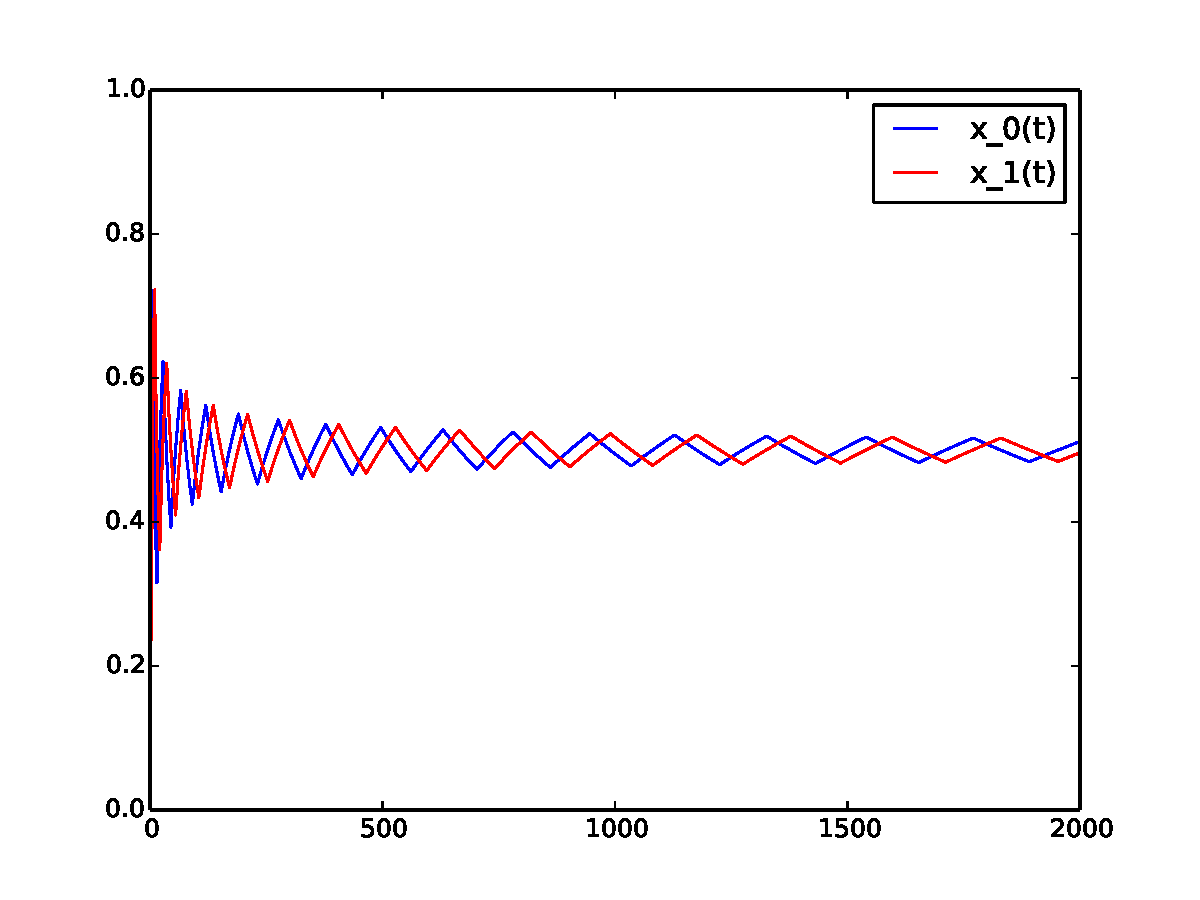
\includegraphics[width=8cm]{fictitious1.pdf}
 \end{center}
 \begin{itemize}
  \item 両プレーヤーの信念がどのように推移しているか?
  \item 2000サイクルの``Matching Pennis Game''
 \end{itemize}
\end{frame}

\begin{frame}\frametitle{Figures}
 \begin{center}
  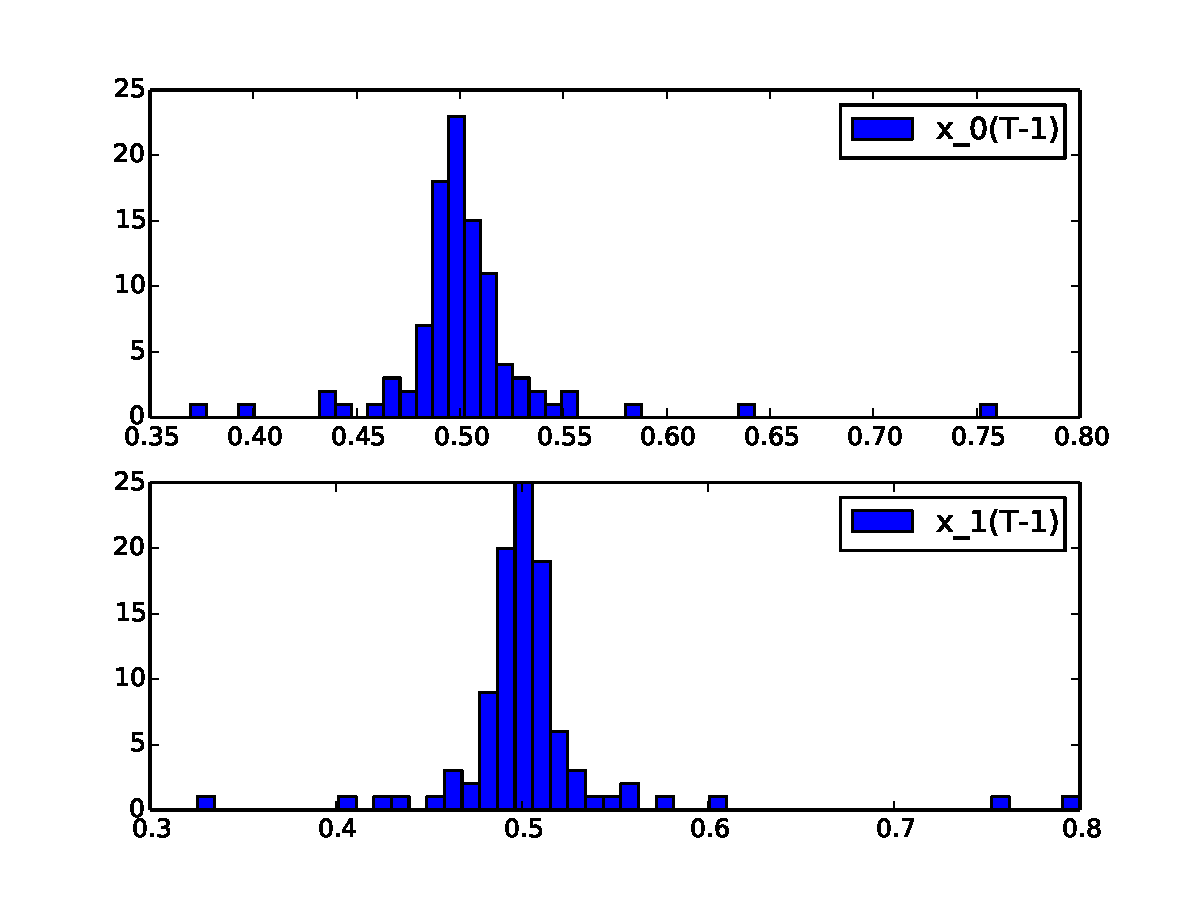
\includegraphics[width=7.5cm]{fictitious_hist0.pdf}
 \end{center}
 \begin{itemize}
  \item プレーヤー0が最終的にそのような信念に辿り着いたのか?
  \item 2000サイクルの``Matching Pennis Game''を100回行って集計
 \end{itemize}
\end{frame}


\subsection{Explanation}
\begin{frame}\frametitle{Explanation of the Code}
 \begin{itemize}
  \item 次のサイクルを繰り返すことで、``Fictitious Play''を実現
  \begin{itemize}
   \item[・] 保持している信念をリストに登録
   \item[・] その信念をもとに期待利得を計算し、その期の行動を決定する
   \item[・] その期における相手の行動を踏まえて、信念を更新
  \end{itemize}
  \item 保持している信念の登録を期首に持ってきている理由
  \begin{itemize}
   \item[→] 初期信念の抜け落ち・最終期に更新された信念の誤登録を防ぐため
  \end{itemize}
 \end{itemize}
\end{frame}

\section{Conclution}
\begin{frame}\frametitle{Conclution : \\Further Improvements}
 \begin{itemize}
  \item 利得表を行列として読み込ませるようにすれば、全体的にスッキリする。
  \begin{itemize}
   \item[・] 期待利得も行列の掛け算で計算可能
  \end{itemize}
  \item 期待利得の計算を行って、その期の行動を決める過程は、関数化すべき
 \end{itemize}
\end{frame}

\end{document}